In der Arbeitsgruppe LARISSA\footnote{\textbf{La}ser \textbf{R}esonance
\textbf{I}onisation \textbf{S}pektroscopy for \textbf{S}elective Tracer
\textbf{A}nalysis} des Instituts für Physik an der Johannes Gutenberg
Universität Mainz wurden über viele Jahre hinweg Methoden zur
Resonanzionisations-Massenspektrometrie (RIMS) entwickelt und verbessert.
Mithilfe dieser Methoden wurden in der Vergangenheit empfindliche und selektive
Ultraspurenbestimmungen verschiedener Elemente der seltenen Erden sowie
vorrangig der radiotoxischen Actinoide durchgeführt. Voraussetzung für die
Ultraspurenanalyse dieser Elemente ist eine möglichst hohe Isotopen- und Isobarenselektivität, welche durch Kombination von elementselektiver resonanter Laserionisation und
isotopenselektiver Quadrupolmassenspektrometrie (QMS) realisiert wird.
Zur Laserionisation werden dabei in der Arbeitsgruppe zwei verschiedene Lasersysteme verwendet, zum einen
gepulst betriebene Titan:Saphir-Laser und zum anderen Kombinationen aus
Dauerstrich-Diodenlasern.\par
Ein wichtiges Teilgebiet dieser Untersuchungen befasst sich mit der
hochauflösenden Ultraspurenanalyse von Uranisotopen (siehe
Nuklidkartenausschnitt Abb.
\ref{fig:uran_nuklidkarte}) mittels HR-RIMS\footnote{\textbf{H}igh
\textbf{R}esolution-RIMS}.
\begin{figure}[h]
 	\centering
 	\fbox{\parbox{\dimexpr \linewidth - 2\fboxrule - 2\fboxsep}{
 	\centering
	    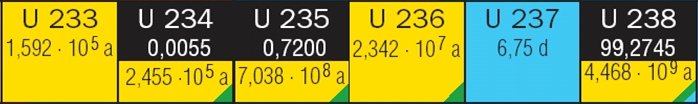
\includegraphics[width=\textwidth-5cm]{gfx/uran_nuklidkarte}
	}}
	\caption[Gesamter experimenteller Aufbau,
	schematisch]{Ausschnitt der Karlsruher Nuklidkarte für langlebige
	Uranisotope \cite{nuklidkarte}.}\label{fig:uran_nuklidkarte}
\end{figure}
Das Schwermetall Uran ist das schwerste natürlich vorkommende Element auf der
Erde mit den beiden dominanten quasi-stabilen Isotopen $^{238}$U und $^{235}$U.
Da $^{238}$U und $^{235}$U in der Natur nicht aus anderen Elementen nachgebildet werden können, lassen sich aus dem durch die Lebenszeiten ermittelbaren natürlichen Isotopenverhältnis
$\nicefrac{^{235}\text{U}}{^{238}\text{U}}=0,00725$ Rückschlüsse auf die
Entstehungszeit unseres Sonnensystems ziehen. Das dritte quasi-stabile Isotop $^{234}$U resultiert aus
$\alpha$-$2\beta$-Zerfällen von $^{238}$U. Das weitere langlebige Isotop
$^{236}$U entsteht durch Einfang thermischer Neutronen aus $^{235}$U. Im
natürlichen Gleichgewicht resultieren Isotopenverhältnisse von
$\nicefrac{^{236}\text{U}}{^{238}\text{U}}=10^{-14}$ aus Neutronenflüssen der
kosmischen Strahlung \cite{Richter1999}. Da in Kernreaktoren sehr hohe
Neutronenflüsse herrschen, können dort wesentlich höhere
$\nicefrac{^{236}\text{U}}{^{238}\text{U}}$-Isotopenverhältnisse bis hinauf zu
$1,4\cdot10^{-4}$ erzielt werden. Die Abweichung vom natürlichen Verhältnis kann
also als Referenz dienen, um einen anthropogenen Eintrag von Uran in die Umwelt nachzuweisen.\par
Eine Obergrenze für die unbedenkliche Aufnahmerate von Uran liegt
bei $0,6\,$\textmu g pro Tag und kg Körpergewicht, wobei das Grund- bzw.
Trinkwasser mit $10^{-6}\,\nicefrac{\text{g}}{\text{l}}$ belastet ist
\cite{who:2005}. Die Überhöhungen der natürlichen Verhältnisse von 
$\nicefrac{^{236}\text{U}}{^{238}\text{U}}$ resultieren maßgeblich aus
Nuklearwaffentests bis einschließlich 1998 und nicht zuletzt aus Reaktorunfällen
wie der bekannte "`Tschernobyl-Unfall"' oder der aktuell brisante Unfall in
Fukushima, Japan. Da die Kontamination der Umwelt großflächig verteilt und stark
verdünnt sein kann, ist es notwendig, sehr kleine Isotopenverhältnisse messen zu
können. Die HR-RIMS bietet hierfür hervorragende Möglichkeiten. Die große
Wichtigkeit dieses Nachweises ist in der Tatsache begründet, dass die Aufnahme von Uran in den Körper toxisch
wirkt und durch die kurzlebigen Uranisotope eine erhöhte Strahlenbelastung
gegeben ist.\par
Um mithilfe von Lasern nicht nur elementselektiv, sondern auch
isotopenselektiv ionisieren zu können\footnote{Isotopieverschiebung, siehe
\ref{subsec:isotopieverschiebung}} und hochauflösende Spektroskopie zu
betreiben, wird sehr schmalbandiges Laserlicht benötigt, welches mit
Dauerstrichlasern erzeugt werden kann. Diodenlaser sind für diesen Einsatz eine
optimale und kostengünstige Lösung. Da die Übergangslinien bei Benutzung von
schmalbandigen Diodenlasern teilweise ebenfalls nur wenige MHz Breite aufweisen,
ist eine aktive Frequenzstabilisierung der Laser unabdingbar.\par
Im Rahmen dieser Diplomarbeit soll eine Frequenzstabilisierung für ein
Diodenlasersystem entwickelt und für den Einsatz zur HR-RIMS an Uran charakterisiert werden.
Folgende Anforderungen werden an das Lasersystem und die Stabilisierung gestellt:
\begin{setlength}{\leftmargini}{1cm}
	\begin{description}
		\item[Stabilität und Frequenzsicherheit]\hfill\\
			Die Laser sollen sowohl auf langen als auch kurzen Zeitskalen (wenige ms bis
			einige Stunden) stabil auf ihrer Frequenz gehalten werden. Die
			Kurzzeitstabilität wird gefordert, um laserinduzierte Zählratenfluktuationen
			zu minimieren. Dabei sind Frequenzfluktuationen von deutlich weniger als
			$10\,$MHz angestrebt. Langzeitdrifts sollen völlig eliminiert werden, um auch
			über lange Zeiten angelegte Messungen reproduzierbar durchführen zu können.
			Dabei ist es wichtig, dass die Stabilisierung ausfallsicher implementiert wird, was
			fehlerfreie Detektion von Frequenzabständen und präzise Steuerung der Laser
			voraussetzt.
		\item[gezielte Frequenzverstimmung]\hfill\\
			Um gezielt atomare Übergangsfrequenzen anfahren und spektroskopische
			Messungen durchführen zu können, soll die Möglichkeit der individuellen
			Laserfrequenzverstimmung implementiert werden. Insbesondere bei
			Isotopenverhältnismessungen ist ein regelmäßiger Wechsel der
			Anregungsschritte verschiedener Uranisotope notwendig.
		\item[Geschwindigkeit]\hfill\\
			Zur Steigerung der Messeffizienz wird angestrebt, Frequenzverstimmungen
			möglichst schnell abzuwickeln. Frequenzverstimmungen von einigen
			GHz sollen innerhalb weniger Sekunden vollzogen werden, um speziell kleine
			Probenmengen möglichst effizient nutzen zu können.
		\item[Automatisierung]\hfill\\
			Um Messungen präzise, systematisch und reproduzierbar durchführen zu
			können, soll die Steuerung der Laser - soweit möglich - vollständig
			automatisiert werden, wobei als Schnittstelle zum Experimentator ein PC mit
			einem \textit{Labview}-Programm dienen soll. Neben der Laserkontrolle soll
			auch die Messdatenaufnahme über denselben PC erfolgen.
	\end{description}
\end{setlength} 
Zur Realisierung der Laserstabilisierung wird die bewährte Methode des
\textit{Fringe-Offset-Locking} \cite{kuschnick:2000:diplomarbeit}, basierend auf
einem \textit{scanning FPI}\footnote{\textit{scanning FPI}: ein in der Länge
verstimmbares Fabry-Pérot-Interferometer}, durch eine kommerzielle
Stabilisierungstechnik, basierend auf einem festen Quadraturinterferometer,
ergänzt.\par
Der Inhalt dieser Arbeit soll die Entwicklung und den Aufbau des Lasersystems,
der optischen Komponenten der Frequenzstabilisierung inklusive Elektronik, die
Programmierung der Software zur Stabilisierung und Experimentsteuerung und die
Charakterisierung des Gesamtsystems umfassen.
